% This is samplepaper.tex, a sample chapter demonstrating the
% LLNCS macro package for Springer Computer Science proceedings;
% Version 2.20 of 2017/10/04
%
\documentclass[runningheads]{llncs}
%\pagestyle{plain}
%
\usepackage{graphicx}
% Used for displaying a sample figure. If possible, figure files should
% be included in EPS format.
%
% If you use the hyperref package, please uncomment the following line
% to display URLs in blue roman font according to Springer's eBook style:
% \renewcommand\UrlFont{\color{blue}\rmfamily}

\usepackage{amssymb}
\usepackage[super]{nth}
\newcommand{\ith}{i\textsuperscript{th} }
\usepackage{algorithm}
\usepackage{algorithmicx}
\usepackage{algpseudocode}
\usepackage{multirow}
\usepackage{amsmath}
\usepackage{extarrows}
\usepackage{pgf}
\usepackage{tikz}
%\usetikzlibrary{arrows,shapes,snakes,automata,backgrounds,petri}

%usepackage{algpseudocode}
%\algdef{SE}[DOWHILE]{Do}{doWhile}{\algorithmicdo}[1]{\algorithmicwhile\ #1}%

\newcommand{\Prob}{\text{Prob}}
\newcommand{\Cor}{\text{Cor}}
\newcommand{\EDP}{\text{EDP}}
\newcommand{\ELP}{\text{ELP}}
\newcommand{\Exp}{\text{Exp}}
\newcommand{\calE}{\mathcal{E}}
\newcommand{\calP}{\mathcal{P}}
\newcommand{\calH}{\mathcal{H}}
\newcommand{\true}{\text{true}}
\newcommand{\false}{\text{false}}
\newcommand{\rotr}{\text{rotr}}
\newcommand{\rotl}{\text{rotl}}
\makeatletter
\newenvironment{breakablealgorithm}
  {% \begin{breakablealgorithm}
   \begin{center}
     \refstepcounter{algorithm}% New algorithm
     \hrule height.8pt depth0pt \kern2pt% \@fs@pre for \@fs@ruled
     \renewcommand{\caption}[2][\relax]{% Make a new \caption
       {\raggedright\textbf{\ALG@name~\thealgorithm} ##2\par}%
       \ifx\relax##1\relax % #1 is \relax
         \addcontentsline{loa}{algorithm}{\protect\numberline{\thealgorithm}##2}%
       \else % #1 is not \relax
         \addcontentsline{loa}{algorithm}{\protect\numberline{\thealgorithm}##1}%
       \fi
       \kern2pt\hrule\kern2pt
     }
  }{% \end{breakablealgorithm}
     \kern2pt\hrule\relax% \@fs@post for \@fs@ruled
   \end{center}
  }
\makeatother

\begin{document}
%
\title{An Automatic Search Tool for Iterative Trails and its Application to estimation of differentials and linear hulls 
%\thanks{Supported by organization x.}
}
%
\titlerunning{An Automatic Search Tool for Iterative Trails}
% If the paper title is too long for the running head, you can set
% an abbreviated paper title here
%
\author{Tianyou Ding\inst{1,2}
%\orcidID{0000-1111-2222-3333} 
\and Wentao Zhang\inst{1,2}
\and Chunning Zhou\inst{1,2}
\and Fulei Ji\inst{1,2}
}
%
\authorrunning{Tianyou Ding et al.}
% First names are abbreviated in the running head.
% If there are more than two authors, 'et al.' is used.
%
\institute{State Key Laboratory of Information Security, Institute of Information Engineering, Chinese Academy of Sciences, Beijing, China\\
\email{\{dingtianyou, zhangwentao, zhouchunning, jifulei\}@iie.ac.cn}
\and School of Cyber Security, University of Chinese Academy of Sciences, Beijing, China
}
%
\maketitle              % typeset the header of the contribution
%
\begin{abstract}

The design and cryptanalysis are the both sides from which we look at symmetric-key primitives. If a symmetric-key primitive is broken by a kind of cryptanalysis, it's definitely insecure. If a designer claims a symmetric-key primitive to be secure, one should demonstrate that the primitive resists against all known attacks. Differential and linear cryptanalysis are two of the most important kinds of cryptanalysis. To conduct a successful differential (linear) cryptanalysis, a differential (linear) distinguisher with significant differential probability (linear correlation) is needed. 

We observe that, for some lightweight symmetric-key primitives, their significant trails usually contain iterative trails. In this work, We propose an automatic tool for searching iterative trails. We model the problem of searching itrative trails to a graph problem. And we find that the combination of iterative trails results in stronger differential and linear propagations. Based on iterative trails, we further propose a method to estimate the probability (correlation) of a differential (linear hull). 

We apply our methods to the 256-bit KNOT permutation, PRESENT, GIFT-64 and RECTANGLE. Iterative trails are found and visualized. If iterative trails are found, our method can efficiently find good differentials and linear hulls. What's more, the results imply that for the primitives we experiment with bit permutations as their linear layers, the best differentials and linear hulls are dominated by iterative trails. 

%An upper bound of the weight of the best trail with arbitrary rounds is obtained in several seconds. When the number of rounds is large, it's illustrated that the upper bound coincide with the best weight or is very tight. An upper bound of the weight of the best differential or linear propagation is also obtained by considering the clustering effect. For 14-round 256-bit KNOT permutation, 13-round GIFT-64 and 15-round RECTANGLE, better differential distinguishers than the best differential trails are obtained. For 10-round 256-bit KNOT permutation and 13-round RECTANGLE, better linear distinguishers than the best linear trails are obtained. Additionally, by constraining the input and output differences and masks, results for KNOT-AEAD fitting certain differential and linear attack scenarios in Duplex mode of operations are obtained. 

\keywords{Differential Cryptanalysis \and Linear Cryptanalysis \and Automatic Search Tools \and Iterative Trails \and Lightweight Cryptography}
\end{abstract}

\section{Introduction}

Differential cryptanalysis (DC) \cite{BS91,BS92} and linear cryptanalysis (LC) \cite{M93,M94_1} are two of the most powerful attacks against modern block ciphers. In 1990, Biham and Shamir introduced differential cryptanalysis and successfully attacked the full-round DES\cite{BS92}. In 1991, they improved the attack with $2^{47}$ chosen plaintexts\cite{BS92}. In 1993, Matsui introduced linear cryptanalysis and succeeded in breaking DES with $2^{47}$ known plaintexts\cite{M93}. In 1994, Matsui improved the data complexity to $2^{43}$\cite{M94_1}. Cryptanalysis also drives the design of ciphers in return. In 2001, Rijmen and Daemon proposed the wide trail design strategy\cite{DR01}, providing provable security against DC and LC for AES winner Rijndael\cite{DR98}. With increasing number of symmetric cryptographic primitives emerging, every well-designed block cipher must resist against DC and LC in the first place. To conduct the differential or linear attack, an adversary expects to find exploitable differential or linear distinguishers. Usually, the probability of the best differential trail and the correlation (or bias) of the best linear trail are respectively used as the indices to the resistance against DC and LC. The two main kinds of the automatic search tools for the best differential and linear trails are dedicated tree search algorithms \cite{M94_2,OMA95,AKM97,BZL14} and mathematical-solver-based methods \cite{MWG12,SHW14-1,SHW14-2,ZZDX19}. In this article, we focus on the dedicated search algorithms. 

In 1994, Matsui proposed a branch-and-bound depth-first tree search algorithm for searching the best differential or linear trail of DES\cite{M94_2}. In 1995, Moriai et al. introduced the concept of search pattern to reduce unnecessary search candidates, which improves the performance of searching the best trail of FEAL\cite{OMA95}. In 1997, Aoki et al. further improved the performance by using a pre-search for impossible search patterns\cite{AKM97}. In 2014, Bao et al. proposed new strategies including starting from the narrowest point, concretizing and grouping search patterns and trailing in minimal changes order, achieving significant efficiency improvement on NOEKEON and Spongent\cite{BZL14}. Dobraunig et al. \cite{DEM15} proposed a stack-based depth-first search algorithm characterizing in guessing sbox by sbox or bit by bit instead of round by round in Matsui's algorithm. Hall-Andersen et al. \cite{HV18} modeled the trail search as a graph problem and managed to obtain results on clustering effect for many ciphers. 

%Another line of research is modelling the differential or linear propagation and solve the model using mathematical tools. In 2011, Wu et al. modeled block ciphers using integer programming\cite{WW11}. Works that modelling using mixed integer linear programming (MILP) include but not limited to \cite{MWG12}. Works that modelling using SAT/SMT include but not limited to []. Works that modelling using constraint programming (CP) include but not limited to [].
Besides automatically searching the best differential or linear trail, iterative trails are used to construct long-round significant trails in order to efficiently obtain exploitable trails for cryptanalysis. Iterative trails refer to trails that have the same input and output difference (or mask) and thus they can concatenate to themselves. Biham and Shamir used iterative differential characteristics to cryptanalyze DES with an arbitrary number of rounds\cite{BS91,BS92}. Knudsen examined the 2 iterative characteristics found in \cite{BS91,BS92} and found additional 3 iterative characteristics for DES\cite{K92}. Wang et al. found a 4-round iterative differential characteristic for PRESENT by which a 14-round significant differential characteristic is constructed\cite{W08}. 
%If the iterative structure is not too complicated, our method is able to find all iterative trails in seconds. Using the iterative structure, We can further determine the weight of the best $n$-round trails constructed by iterative trails. 

%\begin{table}
%	\caption{results on weights of best trails and clusters}\label{tab:sum}
%	\centering
%	\begin{tabular}{|c|c|c|c|c|c|}
%        \hline
%        cipher&target&round&best weight&method&time\\
%        \hline
%        \multirow{9}{*}{KNOT-perm-256}
%        &differential trail   &14     &71         &\cite{ZDY19}           &-\\
%        &differential cluster  &14     &$\leq$ 65.4493    &Sec. \ref{sec:para3}   &511s\\
%        &differential trail   &48     &252         &\cite{BZL14}           &2.87h\\
%        &differential trail   &48     &$\leq$ 252        &Sec. \ref{sec:para2}   &0.1s\\
%        \cline{2-6}
%        &linear trail         &10     &23         &\cite{ZDY19}            &-\\
%        &linear cluster        &10     &$\leq$ 21.8301    &Sec. \ref{sec:para3}   &7509s\\
%        &linear trail         &39     &110         &\cite{BZL14}            &344.01h\\
%        &linear trail         &39     &$\leq$ 110        &Sec. \ref{sec:para2}   &0.6s\\
%        &linear trail         &44     &$\leq$ 125        &Sec. \ref{sec:para2}   &0.6s\\
%        \hline
%        \multirow{4}{*}{PRESENT}
%        &differential trail   &14     &62         &\cite{ZZDX19}          &-\\
%        &differential trail   &14     &$\leq$ 62         &Sec. \ref{sec:para2}   &0.6s\\
%        \cline{2-6}
%        &linear trail     &16     &30         &\cite{ZZDX19}          &-\\
%        &linear trail      &16     &$\leq$ 30         &Sec. \ref{sec:para2}   &0.1s\\
%        \hline
%        \multirow{5}{*}{GIFT-64}
%        &differential trail   &13     &62         &\cite{ZZDX19}          &-\\
%        &differential trail   &13     &$\leq$ 62         &Sec. \ref{sec:para2}   &0.3s\\
%        &differential cluster   &13     &$\leq$ 60.415     &Sec. \ref{sec:para3}   &414s\\
%        \cline{2-6}
%        &linear trail         &12     &31         &\cite{ZZDX19}          &-\\
%        &linear trail         &12     &$\leq$ 32         &Sec. \ref{sec:para2}   &0.2s\\
%        \hline
%        \multirow{6}{*}{RECTANGLE}
%        &differential trail   &14     &61         &\cite{ZBL15}           &-\\
%        &differential trail   &14     &$\leq$ 61         &Sec. \ref{sec:para2}   &1.2s\\
%        &differential cluster   &15     &$\leq$ 63.7857    &Sec. \ref{sec:para3}   &1329s\\
%        \cline{2-6}
%        &linear trail         &13     &31         &\cite{ZBL15}            &-\\
%        &linear trail         &13     &$\leq$ 31         &Sec. \ref{sec:para2}   &0.2s\\
%        &linear cluster ($c^2$)  &13     &$\leq$ 59.3561    &Sec. \ref{sec:para3}   &2481s\\
%        \hline
%	\end{tabular}
%\end{table}

\subsubsection{Our Contribution}
%\begin{enumerate}
%    \item We propose a new automatic tool for searching iterative trails for permutations or block ciphers based on S-boxes. We introduce the concept of $k$-hinge trails by which a directed graph is formed. Inspired by Johnson's algorithm \cite{J75} of finding all the elementary circuits of a directed graph, we find all iterative trails constructed by \textbf{$k$-hinge trails}. We call the directed graph that formed by all iterative trails found \textbf{iterative structure}. Extending a \textbf{general iterative trail} both forward and backward, we obtain the weight of the best trail constructed by iterative trails and the weight of the best differential or linear propagation composed of significant trails constructed by iterative trails. 
%    \item For 256-bit KNOT permutation, PRESENT, GIFT-64 and RECTANGLE, we obtain and visualize the iterative trails, by which we hope to get some insights of symmetric-key primitives with weak diffusion, especially, bit permutation as a diffustion layer. For ASCON permutation, we find that its differential iterative structure based on $3$-hinge trails is empty, which illustrates that ASCON permutation doesn't have iterative differential trails with no more than 3 active S-boxes in each round. 
%    \item For arbitrary-round the 256-bit KNOT permutation, PRESENT, GIFT-64 and RECTANGLE, we obtain the weight of the best trails constructed by iterative trails, which is an upper bound of the weight of the best trails. The upper bound is tight when the round number is large. Our method finishes in several seconds. Comparing our results for the 256-bit KNOT permutation with the results obtained using the method proposed by Bao et al. \cite{BZL14}, we find that the upper bound is exactly the best weight and the time our method consumes is negligible. See Table \ref{tab:sum}. 
%    \item For 256-bit KNOT permutation, GIFT-64 and RECTANGLE, we obtain the weight of the best differential or linear propagation composed of significant trails constructed by iterative trails. Because GIFT-64 and RECTANGLE are keyed block ciphers, the correlation potential ($\sum c^2$) is computed for a cluster of linear trails, while because KNOT permutations are permutations without key xor, the correlation contribution ($\sum c$) is computed for a cluster of linear trails. Except for linear cryptanalysis of GIFT-64, we obtain better weight of the best differential or linear propagation than the weight of the best single trail. See Table \ref{tab:sum}. 
%    \item For different versions of KNOT-AEAD, we obtain the upper bound of the weight of the best trails with input and output differences or masks constrained depending on different attack scenarios. The differential and linear attacks proposed are universally applicable for any AEAD scheme based on the Duplex mode of operations. 
%\end{enumerate}

\subsubsection{Organization}
%The paper is organized as follows. Section \ref{sec:pre} introduces some concepts and notations. Section \ref{sec:para1} gives the algorithm that computes the iterative structure. Section \ref{sec:para2} gives the algorithm that determines the weight of the best trail constructed by iterative trails. Section \ref{sec:para3} gives the algorithm that determine the weight of the best differential or linear propagation composed of significant trails constructed by iterative trails. Section \ref{sec:expe} gives experimental results. In Section \ref{sec:conc}, we conclude the paper. In Appendix \ref{sec:is}, iterative structures are illustrated. 

\section{Preliminaries\label{sec:pre}}

A block cipher is a function $\calE:\bbF_2^k \times \bbF_2^n \rightarrow \bbF_2^n$ with $C=\calE(K,P)$ where $K$, $P$ and $C$ are the $k$-bit master key, $n$-bit plaintext and $n$-bit ciphertext. $k$ is the key size and $n$ is the block size. Embedded into an operation mode, a block cipher can be used to encrypt a message with arbitrary length. 

A permutation is a function $\calP:\bbF_2^n \rightarrow \bbF_2^n$ with $SO=\calP(SI)$ where $SI$ and $SO$ are the $n$-bit input and output state. The sponge/duplex construction where a permutation is embedded can build various primitives such as a hash function, a stream cipher, a MAC or an authenticated encryption scheme \cite{bertoni2007sponge}. Note that a block cipher with key fixed $\calE_K=\calE(K,\cdot)$ can be seen as a permutation.

In this paper, we focus on symmetric-key primitives including iterated key-alternating block ciphers and permutations of SPN structures. The state of such a primitive can be seperated into $m$ words of $s$ bits and it holds that $n=s\times m$. The round function of the $i$-th round consists of three layers and is denoted by $\calR_i=\calL\circ\calS\circ\calA_{W_i}$ where the three layers are:
\begin{itemize}
    \item Addition layer $\calA_{W_i}$: xor the $i$-th $n$-bit round key or constant $W_i$ to the state;
    \item Non-linear layer $\calS$: apply $m$ parallel $s$-bit S-boxes to the words, i.e.
    \begin{align*}
        \calS=\calS_0||\cdots||\calS_{m-1};
    \end{align*}
    \item Linear layer $\calL$: multiply an $n\times n$ bijective binary matrix to the state. 
\end{itemize}
\begin{figure}[H]
    \centering
\begin{tikzpicture}
    \tikzstyle{every node}=[transform shape];
    \tikzstyle{every node}=[node distance=1.2cm];
    \tikzstyle{every node}=[font=\footnotesize,scale=0.9]
    \node (P) [] {$P(SI)$};
    \node (XOR-0) [right of=P,XOR] {};
    \node (S-0) [right of=XOR-0,draw,rectangle] {$\calS$};
    \node (L-0) [right of=S-0,draw,rectangle] {$\calL$};
    \node (XOR-1) [right of=L-0,XOR] {};
    \node (S-1) [right of=XOR-1,draw,rectangle] {$\calS$};
    \node (L-1) [right of=S-1,draw,rectangle] {$\calL$};
    \node (dots) [right of=L-1,] {$\dots$};
    \node (XOR-r-1) [right of=dots,XOR] {};
    \node (S-r-1) [right of=XOR-r-1,draw,rectangle] {$\calS$};
    \node (L-r-1) [right of=S-r-1,draw,rectangle] {$\calL$};
    \node (XOR-r) [right of=L-r-1,XOR] {};
    \node (C) [right of=XOR-r] {$C(SO)$};
    
    \path[line] (P) edge (XOR-0);
    \path[line] (XOR-0) edge node[above] {$X_0$} (S-0);
    \path[line] (S-0) edge node[above] {$Y_0$} (L-0);
    \path[line] (L-0) edge node[above] {$Z_0$} (XOR-1);
    \path[line] (XOR-1) edge node[above] {$X_1$} (S-1);
    \path[line] (S-1) edge node[above] {$Y_1$} (L-1);
    \path[line] (L-1) edge node[above] {$Z_1$} (dots);
    \path[line] (dots) edge node[above] {$Z_{r-2}$} (XOR-r-1);
    \path[line] (XOR-r-1) edge node[above] {$X_{r-1}$} (S-r-1);
    \path[line] (S-r-1) edge node[above] {$Y_{r-1}$} (L-r-1);
    \path[line] (L-r-1) edge node[above] {$Z_{r-1}$} (XOR-r);
    \path[line] (XOR-r) edge (C);

    \node (W-0) [above of=XOR-0] {$W_0$};
    \node (W-1) [above of=XOR-1] {$W_1$};
    \node (W-r-1) [above of=XOR-r-1] {$W_{r-1}$};
    \node (W-r) [above of=XOR-r] {$W_r$};

    \path[line] (W-0) edge (XOR-0);
    \path[line] (W-1) edge (XOR-1);
    \path[line] (W-r-1) edge (XOR-r-1);
    \path[line] (W-r) edge (XOR-r);

    \draw [decorate,decoration={brace,amplitude=5pt,mirror},xshift=-0.5cm,yshift=0pt] (1.2,-0.5) -- ++(2.3,0) node [black,midway,yshift=-0.5cm] {$\calR_0$};
    \draw [decorate,decoration={brace,amplitude=5pt,mirror},xshift=-0.5cm,yshift=0pt] (3.9,-0.5) -- ++(2.3,0) node [black,midway,yshift=-0.5cm] {$\calR_1$};
    \draw [decorate,decoration={brace,amplitude=5pt,mirror},xshift=-0.5cm,yshift=0pt] (7.5,-0.5) -- ++(2.3,0) node [black,midway,yshift=-0.5cm] {$\calR_{r-1}$};

    \draw [decorate,decoration={brace,amplitude=5pt},xshift=-0.5cm,yshift=0pt] (2.1,0.5) -- ++(1.3,0) node [black,midway,yshift=0.5cm] {$\calR_0^*$};
    \draw [decorate,decoration={brace,amplitude=5pt},xshift=-0.5cm,yshift=0pt] (4.8,0.5) -- ++(1.3,0) node [black,midway,yshift=0.5cm] {$\calR_1^*$};
    \draw [decorate,decoration={brace,amplitude=5pt},xshift=-0.5cm,yshift=0pt] (8.4,0.5) -- ++(1.3,0) node [black,midway,yshift=0.5cm] {$\calR_{r-1}^*$};

    %\draw [decorate,decoration={brace,amplitude=10pt,mirror},xshift=-0.5cm,yshift=0pt] (XOR-0.south west) -- node [black,midway,yshift=-0.7cm] {$\calR_0$} (L-0.south east);
    %\draw [decorate,decoration={brace,amplitude=10pt,mirror},xshift=-0.5cm,yshift=0pt] (XOR-1.south west) -- node [black,midway,yshift=-0.7cm] {$\calR_1$} (L-1.south east);
    %\draw [decorate,decoration={brace,amplitude=10pt,mirror},xshift=-0.5cm,yshift=0pt] (XOR-r-1.south west) -- node [black,midway,yshift=-0.7cm] {$\calR_{r-1}$} (L-r-1.south east);

    %\draw [decorate,decoration={brace,amplitude=10pt},xshift=-0.5cm,yshift=0pt] (S-0.north west) -- node [black,midway,yshift=0.7cm] {$\calR_0^*$} (L-0.north east);
    %\draw [decorate,decoration={brace,amplitude=10pt},xshift=-0.5cm,yshift=0pt] (S-1.north west) -- node [black,midway,yshift=0.7cm] {$\calR_1^*$} (L-1.north east);
    %\draw [decorate,decoration={brace,amplitude=10pt},xshift=-0.5cm,yshift=0pt] (S-r-1.north west) -- node [black,midway,yshift=0.7cm] {$\calR_{r-1}^*$} (L-r-1.north east);
\end{tikzpicture}
\caption{Structure of an SPN block cipher or permutation}
\label{fig:SPN}
\end{figure}
We use $W_i$ to denote the $i$-th round key for a block cipher or round constant for a permutation. The primitive iterates the round function several times (See Fig. \ref{fig:SPN}). We denote the $i$-th round function excluding the addition layer by $\calR_i^*=\calL\circ\calS$. We denote the states before the non-linear layer, before the linear layer and after the linear layer of the $i$-th round function by $X_i$, $Y_i$ and $Z_i$. $X_i[j]$ denotes the $j$-th word of $X_i$, i.e. the input value of the $j$-th S-box. For an $X_i$ with $k$ active S-boxes whose index set is $\mathfrak{K}=\{j_0,\cdots,j_{k-1}\}$, we denote it by $X_i[j_0]=x_0,\cdots,X_i[j_{k-1}]=x_{k-1}$ where $x_t\neq 0,\forall 0\leq t<k$ and $X_i[t]=0$ if $t\notin \mathfrak{K}$.

\subsection{Differential Cryptanalysis}

In differential cryptanalysis, the attacker tries to find an exploitable \textit{differential} which is a difference pair $(\Delta P=P\oplus P',\Delta C=C\oplus C')$ with high probability to distinguish the target block cipher or permutation from a random permutation. 

\begin{definition}[Differential Probability of $\calP$]
    For a permutation $\calP$, given $\alpha,\beta\in \bbF_2^n$, the differential probability of the differential $(\alpha,\beta)$ is
    \begin{align*}
        \bbP(\alpha\xrightarrow{\calP}\beta)=2^{-n}\cdot\Big|\{x\in\bbF_2^n|\calP(x)\oplus\calP(x\oplus\alpha)=\beta\}\Big|.
    \end{align*}
\end{definition}

Since the fixed-key block cipher $\calE_K$ is a permutation, its differential probability is also defined as above. However, the key $K$ of $\calE_K$ is unknown for the attacker. Thus the \textit{expected differential probability} (EDP) over all keys is defined.

\begin{definition}[EDP of $\calE$]
    For a block cipher $\calE$, given $\alpha,\beta\in \bbF_2^n$, the EDP of the differential $(\alpha,\beta)$ over a uniformly distributed random key $K\in \bbF_2^k$ is 
    \begin{align*}
        \EDP(\alpha\xrightarrow{\calE}\beta):=2^{-k}\cdot\sum\limits_{K\in \bbF_2^k}\bbP(\alpha\xrightarrow{\calE_K}\beta)
    \end{align*}
\end{definition}

\begin{definition}[Differential Characteristics]
    An $r$-round differential characteristic is a sequence of $r+1$ differences $(\alpha_0,\cdots,\alpha_r)\in(\bbF_2^n)^{r+1}$. Its probability is
    \begin{align*}
        &\bbP(\alpha_0\xrightarrow{\calR_0}\cdots\xrightarrow{\calR_{r-1}}\alpha_r)\\
        =&2^{-n}\cdot\Big|\{x\in\bbF_2^n|\forall i, \calR_i\circ\cdots\circ\calR_0(x)\oplus\calR_i\circ\cdots\circ\calR_0(x\oplus\alpha_0)=\alpha_{i+1}\}\Big|\\
    \end{align*}
\end{definition}

Under the assumption of independent random round keys and the hypothesis of stochastic equivalence \cite{lai1991markov}, the probability of a differential characteristic is calculated round by round and S-box by S-box:
\begin{align*}
    \bbP(\alpha_0\xrightarrow{\calR_0}\cdots\xrightarrow{\calR_{r-1}}\alpha_r)
    =&\prod\limits_{i=0}^{r-1}\bbP(\alpha_i\xrightarrow{\calR_i^*}\alpha_{i+1})\\
    =&\prod\limits_{i=0}^{r-1}\prod\limits_{j=0}^{m-1}\bbP(\alpha_i[j]\xrightarrow{\calS_i}\beta_i[j])
\end{align*}
where $\alpha_{i+1}=\calL(\beta_i),0\leq i<r$. 

The probability of a differential is calculated by summing the probabilities of all differential characteristics sharing the same input and output differences:
\begin{align*}
    \bbP(\alpha\xrightarrow{\calP}\beta) \text{ or } \EDP(\alpha\xrightarrow{\calE}\beta)=&\sum\limits_{\alpha_1,\cdots,\alpha_{r-1}}\bbP(\alpha_0\xrightarrow{\calR_0}\cdots\xrightarrow{\calR_{r-1}}\alpha_r)\\
    =&\sum\limits_{\alpha_1,\cdots,\alpha_{r-1}}\prod\limits_{i=0}^{r-1}\prod\limits_{j=0}^{m-1}\bbP(\alpha_i[j]\xrightarrow{\calS_i}\beta_i[j])
\end{align*}

\subsubsection{Truncated Differential}
Let $\lambda$ be a linear function corresponding to an $n\times l$ binary matrix $M$. The probability of a \textit{truncated} differential of $\lambda\circ\calP$ is given by \cite{daemen2002design}:
\[
    \bbP(\alpha\xrightarrow{\lambda\circ\calP}\beta)=\sum\limits_{\omega|\beta=M\omega}\bbP(\alpha\xrightarrow{\calP}\omega).
\]

\subsection{Linear Cryptanalysis}

In linear cryptanalysis, the attacker tries to find an exploitable \textit{linear approximation}  $\Gamma P\cdot P\oplus \Gamma C\cdot C$ determined by a mask pair $(\Gamma P,\Gamma C)$ revealing an approximate linear relation between $P$ and $C$ and thus distinguishing the target block cipher or permutation from a random permutation. 

\begin{definition}[Correlation]
    The correlation of a Boolean function $f:\bbF_2^n\rightarrow\bbF_2$ is
    \begin{align*}
        c_f=2^{-n}\cdot\Big(\Big| \{x\in\bbF_2^n|f(x)=0\} \Big|-\Big| \{x\in\bbF_2^n|f(x)=1\} \Big|\Big)
    \end{align*}
\end{definition}

\begin{definition}[Linear Approximation]
    For a permutation $\calP$, given $\alpha,\beta\in \bbF_2^n$, $\alpha\cdot x\oplus \beta\cdot\calP(x)$ is a linear approximation of $\calP$ and we denote $c_{\alpha\cdot x\oplus \beta\cdot\calP(x)}$ by $\Cor(\alpha\xrightarrow{\calP}\beta)$.
\end{definition}

\begin{definition}[Linear Characteristics]
    An $r$-round linear characteristic is a sequence of $r+1$ masks $(\alpha_0,\cdots,\alpha_r)\in(\bbF_2^n)^{r+1}$. Its correlation is calculated by
    \begin{align*}
        \Cor(\alpha_0\xrightarrow{\calR_0}\cdots\xrightarrow{\calR_{r-1}}\alpha_r)
        =(-1)^{\oplus_{i=0}^r \alpha_i\cdot W_i}\cdot\prod\limits_{i=0}^{r-1}\Cor(\alpha_i\xrightarrow{\calR_i^*}\alpha_{i+1})
    \end{align*}
\end{definition}

In the case of key-alternating block ciphers, the \textit{expected linear potential} (ELP) of a linear approximation is calculated by summing the correlation squares of all linear characteristics sharing the same input and output masks according to Theorem 7.9.1 in \cite{daemen2002design}:
\begin{align*}
    \ELP(\alpha\xrightarrow{\calE}\beta)=&\sum\limits_{\alpha_1,\cdots,\alpha_{r-1}}\Cor^2(\alpha_0\xrightarrow{\calR_0}\cdots\xrightarrow{\calR_{r-1}}\alpha_r)\\
    =&\sum\limits_{\alpha_1,\cdots,\alpha_{r-1}}\Cor^2(\alpha_0\xrightarrow{\calR_0^*}\cdots\xrightarrow{\calR_{r-1}^*}\alpha_r)\\
    =&\sum\limits_{\alpha_1,\cdots,\alpha_{r-1}}\prod\limits_{i=0}^{r-1}\prod\limits_{j=0}^{m-1}\Cor^2(\alpha_i[j]\xrightarrow{\calS_i}\beta_i[j])
\end{align*}
where $\beta_i=\calL^T(\alpha_{i+1}),0\leq i<r$.

In the case of permutations, the correlation of a linear approximation is calculated by the signed sum of correlations all linear characteristics sharing the same input and output masks:
\begin{align*}
    \Cor(\alpha\xrightarrow{\calP}\beta)=&\sum\limits_{\alpha_1,\cdots,\alpha_{r-1}}\Cor(\alpha_0\xrightarrow{\calR_0}\cdots\xrightarrow{\calR_{r-1}}\alpha_r)\\
    =&\sum\limits_{\alpha_1,\cdots,\alpha_{r-1}}\prod\limits_{i=0}^{r-1} (-1)^{\oplus_{i=0}^r \alpha_i\cdot W_i} \prod\limits_{j=0}^{m-1}\Cor(\alpha_i[j]\xrightarrow{\calS_i}\beta_i[j]).
\end{align*}

\subsection{Concepts in Graph Theory}

A \textit{directed graph} $G(V, E)$ consists of a nonempty and finite set of \textit{vertices} $V$ and a set $E$ of ordered pairs of distinct vertices called \textit{edges}. We denote a directed edge from a vertex $u\in V$ to a vertex $v\in V$ by $u\rightarrow v$. $u$ is called the head of the edge and $v$ is called the tail of it. Each edge $u\rightarrow v$ can be associated with a \textit{cost} and it's denoted by $c(u\rightarrow v)$. A \textit{path} $p_{u,v}$ is a sequence of vertices $(u=v_0,v_1,\cdots,v_{k-1},v=v_k)$ such that $v_i\rightarrow v_{i+1}\in E, 0\leq i<k$. The \textit{length} of the path is
\[
    l(p_{u,v})=k,
\]
the \textit{cost} of the path is
\[
    c(p_{u,v})=\prod\limits_{i=1}^{k}c(v_{i-1}\rightarrow v_i).
\]
The \textit{hull} of $(u,v)$ is defined as the set of all paths $p_{u,v}$ leading from $u$ to $v$. More specifically, we define the $k$-length hull of $(u,v)$, denoted by $h^k(u,v)$, as the set of all paths $p_{u,v}$ satisfying $l(p_{u,v})=k$. The cost of $h^k_{u,v}$ is
\[
    c(h^k_{u,v})=\sum\limits_{l(p_{u,v})=k} c(p_{u,v}).
\]

A path $p_{u,u}$ is called a \textit{circuit}. A circuit is \textit{elementary} if no vertex but the first and last appears twice. Two circuits are distinct if one is not a cyclic permutation of the other. An induced subgraph $G'=(V',E')$ is a (maximal) \textit{strong component} of $G$ if for all $u, v\in V'$ there exist paths $p_{uv}$ and $p_{vu}$ and this property holds for no subgraph of $G$ induced by a vertex set $\overline{V'}$ such that $V' \subset \overline{V'} \subseteq V$.

Let $G$ be a directed graph with vertices $V$ and edges $E$. If the vertices in $V$ are partitioned into $l$ subsets $S_0,\cdots,S_{l-1}$, called \textit{stages}, such that any edge in $E$ has the form $u\rightarrow v$ with $u\in S_i$ and $v\in S_{i+1}$, $0\leq i<l$. We call the graph a \textit{multistage graph}.

%\subsubsection{Notation} In this paper, we will not distinguish a vertex from a difference or mask value, an edge from a 1-round trail, a path from a trail, a weight from a differential probability or linear correlation. Note that the term "weight" has several meanings in other literatures, like the hamming weight of a difference or mask value, the negative logarithm of a differential probability or linear correlation. 

\subsection{Estimating EDP and ELP using a Graph Approach}

In \cite{EPRINT:HalVej18}, an algorithm for differential or linear characteristic search is proposed using a multistage graph approach. To summarize, once the onr-round characteristics to be considered are determined, the best differential or linear approximation within the search space can be found. We present its main framework in three steps as follows.

\subsubsection{Generating a multistage graph}
An edge is equivalent to a one-round characteristic. The cost of the edge is determined by the differential probability or correlation of the one-round characteristic. By selecting the interesting one-round characteristics, the multistage graph $G$ is generated by adding corresponding edges between stages $S_i$ and $S_{i+1}, \forall i\in[0,r-1]$. 

\subsubsection{Graph Pruning}
\begin{enumerate}
    \item Remove any vertex in $S_0$ with no outgoing edges.
    \item Remove any vertex in $S_1$ to $S_{r-1}$, if it does not have at least one incoming and one outgong edge, remove it.
    \item Remove any vertex in $S_r$ with no incoming edges.
\end{enumerate}
Repeat the above procedure until no more vertices can be removed. 

\subsubsection{Finding the best differential or linear approximation}
\begin{enumerate}
    \item Let $\calH$ be an empty hash table. Choose an $\alpha\in S_0$ and let $\calH(\alpha)=1$.
    \item For each stage $S_0$ to $S_{r-1}$ of $G$, do:
    \begin{enumerate}
        \item Create an empty hash table $\calH'$.
        \item For each key of $\calH$, let $u$ be the corresponding vertex in $G$. Let $t=\calH(u)$. Then, for each edge $u\rightarrow v$. if $\calH'(v)$ doesn't exists, let $\calH'(v)=t\cdot c(u\rightarrow v)$. Otherwise, let $\calH'(v)=\calH'(v)+t\cdot c(u\rightarrow v)$.
        \item Let $\calH=\calH'$.
    \end{enumerate}
    \item $\calH(\beta)$ now contains $c(h^r_{\alpha,\beta})$.
    \item Repeat for a new value of $\alpha$.
\end{enumerate}
The EDP or ELP for the best differential or linear approximation is estimated by $\max\limits_{\alpha,\beta}c(h^r_{\alpha,\beta})$.
\section{Searching for Iterative Trails and Estimation of Differentials and Linear Hulls\label{sec:method}}

\subsection{Generating a Graph Modelling Difference or Mask Propagations}

In a directed graph, each vertex can be associated with a difference or mask value. Each edge $u\rightarrow v$ represents a 1-round differential or linear trail. Given the round transformation $F$ of an iterative block cipher or permutation $\calE$, in the case of differential cryptanalysis, the weight of an edge is defined as:
\[
    w(u\rightarrow v)=\Prob^{F}(u,v).
\]
In the case of linear cryptanalysis, if $\calE$ is a block cipher, the weight of an edge is defined as:
\[
    w(u\rightarrow v)=(\Cor^{F}(u,v))^2;
\]
else if $\calE$ is a permutation, the weight is defined as:
\[
    w(u\rightarrow v)=\Cor^{F}(u,v).
\]

In this way, a weighted directed graph $G_{F}=(V_{F},E_{F})$ is generated to describe the difference or mask propagations given $F$. A path in the graph represents a differential or linear trail. A hull with length $k$ in the graph represents a differential or linear hull. 

However, the $G_F$ generated is too large for it has $2^n$ vertices. Therefore we need to choose a interesting graph according to computation power. 

In order to limit the size of $V_F$, we set a parameter $max\_asn$ defined as the maximum number of active S-boxes that a vertex can has. Given $\text{Asn}(\cdot)$ as the function that returns the number of active S-boxes of a difference or mask, $G_{F,max\_asn}=(V_{F,max\_asn},E_{F,max\_asn})$ is an induced subgraph of $G_F$ where $V_{F,max\_asn}$ is given by
\[
    V_{F,max\_asn}=\{u|u\in V_F \text{ and } \text{Asn}(u)\leq max\_asn\}.
\]

\subsection{Finding the Best Iterative Trail}\label{sec:fbit}

\begin{definition}[Iterative Trails]\label{def:it}
	A differential or linear trail $(v^{(0)},\cdots,v^{(r)})$ is iterative if $v^{(0)}=v^{(r)}$.
\end{definition}

\begin{definition}[Elementry Iterative Trails]
    An iterative differential or linear trail $(v^{(0)},\cdots,v^{(r)}=v^{(0)})$ is elementary if $v^{(i)}\neq v^{(j)},\forall i,j\in [0,r-1]$.
\end{definition}

According to the definition, Obiviously a (elementary) circuit in the graph represents an (elementary) iterative trail. Applying Johnson's algorithm in \cite{J75}, we can enumerate all elementary circuits in $G_{F,max\_asn}$. The time complexity is $O((n + e)(c + 1))$ and memory complexity is $O(n + e)$, where there are $n$ vertices, $e$ edges and $c$ elementary circuits in the graph.

Once a short-round elementary iterative trails is found, it can be concatenated to itself arbitary times and forms a long-round iterative trail. For a cipher that has iterative trails, the negative logarithm of the largest differential probability or linear correlation increases no faster than a linear function of the round number. 

For an $rd$-round iterative trail with weight $wt$, we regard its weight per round $wt/rd$ as an index describing the weight growth of the iterative trail. We refer the best iterative trail to the one with the largest weight per round. We claim that one of the best iterative trails must be an elementary one. Thus we can find out the best elementary iterative trail
among the ones enumerated by Johnson's algorithm \cite{J75} and evaluate the best weight growth of one single iterative trail. The procedure is given in Algorithm \ref{algo:1} and the details of Johnson's algorithm are given in Appendix. 

\begin{algorithm}
	\caption{Finding the best iterative trail}
	\label{algo:1}
	\begin{algorithmic}[1]
		\Require $G_{F,max\_asn}$
		\Ensure the largest weight per round of an iterative trail
		\Procedure {}{}
		\State $wpr\leftarrow 0$
		\For{each elementary circuit $p'$ in $G_{F,max\_asn}$ enumerated by Johnson's algorithm}
		\If{$w(p')/l(p')>wpr$}
		\State $wpr\leftarrow w(p')/l(p'),p\leftarrow p'$
		\EndIf
		\EndFor
		\State \Return{$wpr$}
		\EndProcedure
	\end{algorithmic}
\end{algorithm}

\subsection{Finding the Best Iterative Hull}\label{sec:fbih}

\begin{example}\label{eg:1}
	Suppose that we find two elementary iterative trails $p_0=u_0\rightarrow u_1\rightarrow u_0$ and $p_1=u_0\rightarrow u_2 \rightarrow u_0$. $p_0$ itself can form a 4-round iterative trail $u_0\rightarrow u_1\rightarrow u_0\rightarrow u_1\rightarrow u_0$ with weight $w^2(p_0)$. Additionally combined with $p_1$, 4 4-round iterative trails can be formed which are
	\begin{align*}
		&u_0\rightarrow u_1\rightarrow u_0\rightarrow u_1\rightarrow u_0\\
		&u_0\rightarrow u_1\rightarrow u_0\rightarrow u_2\rightarrow u_0\\
		&u_0\rightarrow u_2\rightarrow u_0\rightarrow u_1\rightarrow u_0\\
		&u_0\rightarrow u_2\rightarrow u_0\rightarrow u_2\rightarrow u_0.
	\end{align*}
	Thus a 4-round iterative hull containing 4 trails with weight $w^2(p_0)+w^2(p_1)+2w(p_0)w(p_1)$ can be constructed.
\end{example}

From Example \ref{eg:1}, we find that it's not enough to evaluate the best weight growth of one single iterative trail. If two elementary circuits have common vertices, then the combination of elementary iterative trails may result in iterative hulls with better weight growths.  

To evaluate the weight growth of iterative hulls, we define subgraph \textit{iterative structure}. 

\begin{definition}[Iterative Structure]
	An induced subgraph $G'=(V',E')$ is a (maximal) iterative structure of $G$ if for all $u\in V'$, there exist at least one edge originating from it and one edge terminating at it. And this property holds for subgraph of $G$ induced by a vertex set $\overline{V'}$ such that $V' \subset \overline{V'} \subseteq V$.
\end{definition}

We claim that for an arbitary vertex in the iterative structure, it whether belongs to at least one elementary circuit or belongs to at least one path linking two elementary circuits. 

To compute the iterative structure $G^{IS}_{F,max\_asn}$ of $G_{F,max\_asn}$, we eliminate the vertices in having no incoming or outgoing edges until the size of the graph become stable. 

Given the round number $r$, we can compute $w(h_{u,v}^r)$ for all $u,v$ in $V^{IS}_{F,max\_asn}$. For a sufficient large $r$, we regard $\max\limits_{u,v}w(h_{u,v}^r)/r$ as an index describing the best weight growth of the iterative hull. The procedure is given in Algorithm \ref{algo:2}.

\begin{algorithm}
	\caption{Finding the best iterative hull}
	\label{algo:2}
	\begin{algorithmic}[1]
		\Require $G_{F,max\_asn}$, the number of rounds $r$
		\Ensure the largest weight per round of an $r$-round hull in the iterative structure
		\Procedure {}{}
		\State Eliminate all vertices having no incoming or outgoing edges repeatedly until no more vertices can be eliminated and restore the subgraph into $G^{IS}_{F,max\_asn}$
		\State Let $\mathcal{H}$ be a hash table. Set $\mathcal{H}(u,v)\leftarrow 0$ for all $u,v\in V^{IS}_{F,max\_asn}$
		\For{$i=1:r$}
		\State Create a new hash table $\mathcal{H}'$. 
		\For{each pair of keys $(u,v)$ of $\mathcal{H}$}
		\For{each edge $v\rightarrow x$ originating from $v$ in $G^{IS}_{F,max\_asn}$}
		\State $\mathcal{H}'(u,x)\leftarrow \mathcal{H}'(u,x)+\mathcal{H}(u,v)\cdot w(v\rightarrow x)$
		\EndFor
		\EndFor
		\State $\mathcal{H}\leftarrow \mathcal{H}'$
		\EndFor
		\State \Return{$\max\limits_{u,v}\mathcal{H}(u,v)$}
		\EndProcedure
	\end{algorithmic}
\end{algorithm}

\subsection{Finding the Best Differential or Linear Hull}\label{sec:fbh}

In \cite{W08}, a 4-round elementary iterative trail is found and is used to construct a 12-round iterative trail. By further extending the trail forward and backward by one round, a 14-round trail is obtained. 

Following this idea, we first generate a multi-stage graph according to $G^{IS}_{F,max\_asn}$ and extend both forward and backward from each vertex in $V^{IS}_{F,max\_asn}$ for several rounds and restore the trails in the multi-stage graph. Then we compute the weight stage by stage. The procedure is given in Algorithm \ref{algo:3}

\begin{algorithm}
	\caption{Finding the best differential or linear hull}
	\label{algo:3}
	\begin{algorithmic}[1]
		\Require $G^{IS}_{F,max\_asn}$, the number of rounds $r$, the number of round to be extended $k$, the smallest weight that a single round of a extended trail can has $wlb$
		\Ensure the largest weight of an $r$-round hull
		\Procedure {}{}
		\State Build a graph $MSG$ with $r+1$ stages $S_0,\cdots,S_r$ where $S_i\leftarrow V^{IS}_{F,max\_asn}$. For each edge $u\rightarrow v$ in $E^{IS}_{F,max\_asn}$, we append $u\rightarrow v, u\in S_i,v\in S_{i+1}, \forall i$ to $MSG$. 
		\For{each trail $p=(v_0,v_1,\cdots,v_l)$ extended from a vertex in $V^{IS}_{F,max\_asn}$ with $l\le k$ and $w(v_{i-1}\rightarrow v_i)\ge wlb$}
		\If{$p$ is a trail extended forward from $v_0\in V^{IS}_{F,max\_asn}$}
		\For{$i\leftarrow 1:l$}
		\State Append $v_{i-1}\rightarrow v_i$ between $S_{r-l+i-1}$ and $S_{r-l+i}$
		\EndFor
		\ElsIf{$p$ is a trail extended backward from $v_l\in V^{IS}_{F,max\_asn}$}
		\For{$i\leftarrow 1:l$}
		\State Append $v_{i-1}\rightarrow v_i$ between $S_{i-1}$ and $S_{i}$
		\EndFor
		\EndIf
		\EndFor
		\State Let $\mathcal{H}$ be a hash table. 
		\For{each $u\in S_0$}
		\State $\mathcal{H}(u)\leftarrow 0$
		\For{$i=1:r$}
		\State Create a new hash table $\mathcal{H}'$. 
		\For{each key $v$ of $\mathcal{H}$}
		\For{each edge $v\rightarrow x, v\in S_{i-1},x\in S_i$}
		\State $\mathcal{H}'(x)\leftarrow \mathcal{H}'(x)+\mathcal{H}(v)\cdot w(v\rightarrow x)$
		\EndFor
		\EndFor
		\State $\mathcal{H}\leftarrow \mathcal{H}'$
		\EndFor
		\If{$\max\limits_{v}\mathcal{H}(v)>wt$}
		\State $wt\leftarrow \max\limits_{v}\mathcal{H}(v)$
		\EndIf
		\EndFor
		\State \Return{$wt$}
		\EndProcedure
	\end{algorithmic}
\end{algorithm}


%For any trail based on iterative trails, it can be treated as three parts: the extension backward, the iterative trail and the extension forward. The 14-round differential trail of PRESENT found in \cite{W08} is shown in Table \ref{tab:trail-present}. It is constructed by concatenating a 4-round iterative trail to itself two times and extending both forward and backward by 1 round. Thus the subtrail from round 0 to round 1 is the extension backward part, the one from round 1 to round 13 is the iterative trail part and the one from round 13 to round 14 is the extension forward part. In the following, we try to compute the largest probability a trail of such type can has based on $G^{IT}_{F,max\_asn}$. 

%In another way, a weighted 2-stage graph $G^1_F=(V^1_F,E^1_F)$ can also be generated to describe the 1-round differentials or linear hulls. $G^1_F$ has 2 stages $S_0$ and $S_1$ each being $\mathbb{F}_2^n$. For $u\in S_0$ and $v\in S_1$, the weight of an edge $w^1(u\rightarrow v)$ is defined the same way as $l(u\rightarrow v)$ in $G_F$ is.

%If $S_0=S_1$, then $G^1_F$ can be iteratively concatenated to itself. 


\section{Improvements}\label{sec:improvements}

\subsection{Expanding $G_{F,max\_asn}$}

\begin{definition}[Activity Pattern]
	The activity pattern of a trail $(u^{(0)},u^{(1)}$ $,\cdots,u^{(r)})$ is a sequence $(a_0,a_1,\cdots,a_r)$ where $a_i=\text{Asn}(u^{(i)})$. 
\end{definition}

\begin{definition}[Collective Activity Pattern]
	A trail $(u^{(0)},u^{(1)},\cdots,u^{(r)})$ with activity pattern $(a_0,a_1,\cdots,a_r)$ belongs to collective acticity pattern $(b_0,b_1,\cdots,b_r)$ if $a_i\leq b_i,\forall 0\leq i\le r$. 
\end{definition}

When generating graph $G_{F,max\_asn}$, we only consider trails with collective activity pattern $(max\_asn,max\_asn)$. To get more accurate results on finding best exploitable differentials and linear hulls, search space should be further expanded. Thus when generating $G_{F,max\_asn}$, we can instead consider trails with collective activity pattern $(max\_asn, max\_asn+1, max\_asn)$ or $(max\_asn, max\_asn+1, max\_asn+1, max\_asn)$, etc.

\subsection{Modification in case of Rotation Equivalence}

According to \cite{ZBL15}, RECTANGLE has the property of rotational symmetry, that is, all its operations have rotational symmetry. 

\begin{definition}[Rotational Symmetry and Rotation Equivalence]
	First suppose that a trail $p=(u^{(0)},u^{(1)},\cdots,u^{(r)})$ is found valid. If the cipher is based on SPN structure, the difference or mask value $u^{(i)}$ can be further described by S-boxes as $u^{(i)}=(u_1^{(i)},u_2^{(i)},\cdots,u_k^{(i)})$ where $k$ is the number of S-boxes of each round. If the cipher has rotation equivalence, then another trail $p'=(v^{(0)},v^{(1)},\cdots,v^{(r)})$ is also valid, if there exists $j$ such that $(v_1^{(i)},v_2^{(i)},\cdots,v_k^{(i)})=(u_{j+1}^{(i)},u_{j+2}^{(i)},\cdots,u_{j}^{(i)}),\forall i$. And we call two values $u=(u_1,u_2,\cdots,u_k)$ and $v=(v_1,v_2,\cdots,v_k)$ are rotation equivalent if there exists $j$ such that $(u_1,u_2,\cdots,u_k)=(v_{j+1},v_{j+2},\cdots,v_{j})$. 
\end{definition}

\begin{example}\label{exp:itre}
	Suppose that a cipher $\mathcal{E}$ has rotational symmetry and a 1-round trail $0x3000f000\rightarrow 0x03000f00$ is found. According to Definition \ref{def:it}, it's not an iterative trail. However, it can also be concatenated to itself arbitary times.
\end{example}

From Example \ref{exp:itre}, we can see that if a cipher has rotational symmetry, the definition of iterative trails should be modified as follows:  

\begin{definition}[Iterative Trails under Rotation Equivalence]
	A differential or linear trail $(v^{(0)},\cdots,v^{(r)})$ is iterative if $v^{(0)}$ and $v^{(r)}$ are rotation equivalent.
\end{definition}

The rotation equivalence then defines a rotation equivalent class. In the euivalent class, we define a representive element as follows:

\begin{definition}[Rotation Equivalent Class and Rotation Representive Element]
	A rotation equivalent class is a difference or mask value maximal set that for every two elements $u$ and $v$ in it, we have $u$ and $v$ are ratation equivalent. The representive element of the rotation equivalent class is the largest value in it. The rotation is operated on S-boxes. For any element $u$ in a rotation equivalent class, we call the distance between $u$ and its representive element $u'$ the left rotation number from it to its representive elelent and denote the distance as $d(u)$. 
\end{definition}

We denote the transform from $u=(u_1,u_2,\cdots,u_k)$ to $u'=(u_{j+1},u_{j+2},\cdots,u_{j+k})$ where $u_i$ is the value of the i-th S-box as $\rotl_j(\cdot)$. In the same way, the inverse transfrom is $\rotr_j(\cdot)$. We denote the transform from $u$ to its representive element as $r(\cdot)$. We define $d(u\rightarrow v)=(d(v)-d(u))\mod sn$ where $sn$ is the number of S-boxes. 

In the graph generation of a cipher having rotational symmetry, a vertex representives a rotation equivalent class instead of a value. However, This results in multiple costs of one edge. Or it can be seen as multiple edges between two vertices. 

\begin{example}
	For a cipher having rotational symmetry, suppose that we find two 1-round trails $0x3000f000\rightarrow 0x0e000020$ with weight $2^5$ and $0xf0003000\rightarrow 0xe0000200$ with weight $2^6$, then edge $u=0xf0003000\rightarrow v=0xe0000200$ is appended to the graph. The edge has two costs: $w(u\rightarrow v)=2^5$ when $d(u\rightarrow v)=5$ and $w(u\rightarrow v)=2^6$ when $d(u\rightarrow v)=0$. 
\end{example}

\section{Experiments\label{sec:experiment}}

\subsection{Experiments on Searching for Iterative Trails}

We apply our method in Section \ref{subsec:iterative-trails} to PRESENT, GIFT-64, RECTANGLE, 256-bit KNOT permutation and ASCON permutation. The results on iterative trails are shown in Table \ref{tab:iterative-trails}. The visualizations of $G^{IT}_{F,max\_asn}$ are shown in Appendix \ref{app:visualization}.

%The iterative structures are illustrated in Figures \ref{fig:graph_knot256_ddt}-\ref{fig:graph_gift_lat} in Appendix \ref{sec:is}. The differential and linear iterative structures of PRESENT are too big to be illustrated. The quantitive summary results are illustrated in Table \ref{tab:is}. For PRESENT, we constrain the elementary differential iterative trails within 10 rounds, for the genuine iterative structure is too complicated.

\begin{table}
	\caption{Results on iterative trails}\label{tab:iterative-trails}
	\centering
	\tiny
	\begin{tabular}{|c|c|c|c|c|c|c|c|c|c|}
		\hline
		cryptanalysis & cipher ($F$) & rs. & $max\_asn$ &$|V_{F,max\_asn}|$&$\leq n$& $|V^{IT}_{F,max\_asn}|$ & \#ecs. & best w/l. &time\\
		\hline
		\multirow{5}{*}{differential (Prob.)}
		&KNOT-perm-256 & yes & 2 & 8214 & - & 5 & 6 & 5.3 & 0.3s\\
		\cline{2-10}
		&PRESENT & no & 2 & 17256 & 10 & 225 & 463 & 4.5 & 2.1s\\
		\cline{2-10}
		&GIFT-64 & no & 2 & 19344 & - & 32 & 66 & 5 & 1.8s\\
		\cline{2-10}
		& RECTANGLE & yes & 2 & 1450 & - & 6 & 3 & 5 & 0.1s\\
		\cline{2-10}
		& ASCON-perm & yes & 3 & 3939 & - & 0 & 0 & - & 2.7h\\
		\hline
		\multirow{4}{*}{linear (Cor.)}
		& KNOT-perm-256 & yes & 2 & 8229 & - & 8 & 10 & 3 & 0.4s\\
		\cline{2-10}
		& PRESENT & no & 1 & 208 & - & 27 & 114223 & 2 & 3.6s\\
		\cline{2-10}
		& GIFT-64 & no & 2 & 21696 & - & 16 & 4 & 3 & 2.3s\\
		\cline{2-10}
		& RECTANGLE & yes & 2 & 1465 & - & 10 & 16 & 3 & 0.1s\\
		\cline{2-10}
		& ASCON-perm & yes & 3 & 336 & - & 0 & 0 & - & 4.0h\\
		\hline
		\multicolumn{9}{l}{rs.: whether the cipher has the property of rotational symmetry}\\
		\multicolumn{9}{l}{$\leq n$: the length of any elementary circuit is restricted to no more than $n$}\\
		\multicolumn{9}{l}{\#ecs.: number of elementary circuits}\\
		\multicolumn{9}{l}{best w/l.: the smallest weight/length that an elementary circuit can has}\\
	\end{tabular}
\end{table}

We consider the smallest weight per length an elementary iterative trail can has (best w/l. in Table \ref{tab:iterative-trails}) as an index describing the growth of iterative differential and linear propagations. We can see that PRESENT has both the weakest growth of iterative differential and linear propagations. The weakest differential iterative trail is exactly the one found by Wang et al.\cite{W08}. 

%256-bit KNOT permutation, PRESENT, GIFT-64 and RECTANGLE share a common point that each of them uses a bit permutation as its linear layer which is hardware-friendly and an S-box also providing diffusion as its non-linear layer. However, due to the weakness of the linear layer, the best differential and linear weights of them all increase proportionally with the round number, because of the existence of iterative trails. Meanwhile ASCON permutation uses a low-latency S-box and a strong linear layer. From Table \ref{tab:is} we can see that the differential iterative structure of ASCON permutation is empty even when $k=3$.

%A question is raised that how far a cipher with a comparatively weak diffusion layer can go. As long as the iterative structure is not empty, the best weight increases proportionally with the round number. Through the visualization of iterative structure, we hope to inform symmetric-key primitive designers of the detailed structure of iterative trails. 

%\subsection{Results of the Best Weights}
%
%Results for 256-bit KNOT permutation, PRESENT, GIFT-64 and RECTANGLE on the best weights obtained using our methods in section \ref{sec:para2} and \ref{sec:para3} are illustrated in Tables \ref{tab:knot256}-\ref{tab:rect}. They are compared with the weights of the best differential and linear trails. Using the method proposed in section \ref{sec:para2}, we need to determine the parameters $(r^f,r^b)$ first. Using the method proposed in section \ref{sec:para3}, we need to determine the parameters $(r^f,w^f,r^b,w^b,gap)$ first, where $gap=wub-bw[r]$ when searching $r$-round clusters. The larger each parameter is, the more time is consumed and the more accurate the result is. 
%
%The results obtained by our method coincide with the results of genuine best weight when the round number is large, except for results of linear weights for GIFT-64. The best 13-round linear trail of GIFT given in \cite{ZZDX19} has correlation $2^{-34}$ and has no iterative trail in it. Our method is unable to find such a trail. 
%
%%Our method finishes in minutes or even in seconds and is able to obtain an upper bound of the best weight for ciphers have iterative trails.

\subsection{Experiments on Finding Differential Trails and Linear Trails}

We apply our method in Section \ref{subsec:find-trails} and \ref{subsec:find-clusters} to PRESENT, GIFT-64, RECTANGLE and 256-bit KNOT permutation. The algorithm is run on an Intel Core i7-6700 CPU at 3.40GHz with 16GB RAM. The results for differential cryptanalysis are shown in Table \ref{tab:EDP}. The results for linear cryptanalysis are shown in Table \ref{tab:ELP}. 

\begin{table}
	\caption{Results for differential cryptanalysis}\label{tab:EDP}
	\centering
	\begin{tabular}{|c|c|c|c|c|c|c|}
		\hline
		cipher & rounds & EDP1 & Time & EDP2 & Time \\
		\hline
		PRESENT & \\
		\hline 
		RECTANGLE & 13 & 56 & 1.2s & 55.6601 & 12007.5s \\
		\hline
		GIFT-64 \\
		\hline
		KNOT-perm-256 \\
		\hline
	\end{tabular}
\end{table}

\begin{table}
	\caption{Results for linear cryptanalysis}\label{tab:ELP}
	\centering
	\begin{tabular}{|c|c|c|c|c|c|c|}
		\hline
		cipher & rounds & ELP1 & Time & ELP2 & Time \\
		\hline
		PRESENT & \\
		\hline 
		RECTANGLE & 13 & 62 & 0.2s & 59.6377 & 337.195s \\
		\hline
		GIFT-64 \\
		\hline
		KNOT-perm-256 \\
		\hline
	\end{tabular}
\end{table}

\subsection{Experiment on KNOT}

\subsubsection{Attack Model 1}


\section{Conclusion\label{sec:conclusion}}

In this work, we propose a new automatic tool searching for iterative trails for symmetric-key primitives based on S-boxes. We visualize the graph representation of iterative trails hoping to provide additional insignts. Based on the iterative trails, we efficiently estimate the probabilities of differentials and correlations of linear hulls. Our results show that the combination of iterative trails is very likely to enhance differential and linear propagations. What's more, our results show that, for ciphers we conduct experiments on with bit permutations as their linear layers, the good differentials and linear hulls are dominated by iterative trails. 

We have conducted an initial study on ASCON permutation. For its comparatively strong diffusion layer, iterative trails are difficult to be found. A question raised for designers is that, whether a cipher with bit permutation as its linear layer can have no iterative trails. And we plan to continue experimenting on ciphers with bit permutations as linear layers like ICEBERG, PUFFIN, etc. Ciphers with Feistel structure, like DES, are also going to be considered. 

In Algorithm \ref{algo:1}, we generate a graph describing the 1-round differential or linear propagations and then shrink it to a subgraph named as an iterative structure. The number of active S-boxes are limited. By using the technique in Section \ref{sec:expansion}, we can take more 1-round differential or linear propagations into consideration. The collection of interesting 1-round differential or linear propagations is heuristic. One may heuristically alter the way of the collection. 

In Algorithm \ref{algo:3}, we build a multistage graph by further considering trails extended from the vertices in the iterative structure. The weight of the trails are bounded in certain heuristic way. One can loose the bounds to obtain more accurate results but costing more time and memory. One can also heuristically alter the way how the bounds restrict the extension trails. 



%
% ---- Bibliography ----
%
% BibTeX users should specify bibliography style 'splncs04'.
% References will then be sorted and formatted in the correct style.
%
\bibliographystyle{splncs04}
\bibliography{mybibliography}
%
\begin{thebibliography}{8}
%\bibitem{ref_article1}
%Author, F.: Article title. Journal \textbf{2}(5), 99--110 (2016)

%\bibitem{ref_lncs1}
%Author, F., Author, S.: Title of a proceedings paper. In: Editor, F., Editor, S. (eds.) CONFERENCE 2016, LNCS, vol. 9999, pp. 1--13. Springer, Heidelberg (2016). \doi{10.10007/1234567890}

%\bibitem{ref_book1}
%Author, F., Author, S., Author, T.: Book title. 2nd edn. Publisher, Location (1999)

%\bibitem{ref_proc1}
%Author, A.-B.: Contribution title. In: 9th International Proceedings on Proceedings, pp. 1--2. Publisher, Location (2010)

%\bibitem{ref_url1}
%LNCS Homepage, \url{http://www.springer.com/lncs}. Last accessed 4 Oct 2017

%%%%%%%%%%%%%%%%%%%%%%%%%%%%%%%%%%%%%%%%%%%%%%%%%%%%%%%%%%%
%dedicated search:
%AKM97,BZL14,OMA95

%MILP search:
%MWG12,SHW14-1,SHW14-2,ZZDX19

%differential cryptanalysis:
%BS91,BS92

%linear cryptanalysis:
%M93,M94_1,M94_2

%ciphers
%Keccack:BDPV12,BDPVV14
%PRESENT:BKL07
%GIFT:BPP17
%Ascon:DEMS16
%AES:DR98,DR01,DR02
%RECTANGLE:ZBL15
%KNOT:ZDY19

%iterative trails
%K92,W08

%algorithms:
%J75,V03

%provable security
%R04
%%%%%%%%%%%%%%%%%%%%%%%%%%%%%%%%%%%%%%%%%%%%%%%%%%%%%%%%%%%

\bibitem{CXQ}
Yaxin Cui, Hong Xu, Wenfeng Qi. An Efficient method to construct Differential and Linear Characteristics of bit-slice block ciphers. (in Chinese). Journal of Cryptologic Research, 2020. Accepted. 

\end{thebibliography}
\appendix

\section{Visualization of Iterative Structures\label{app:visualization}}

\begin{figure}
	\centering
	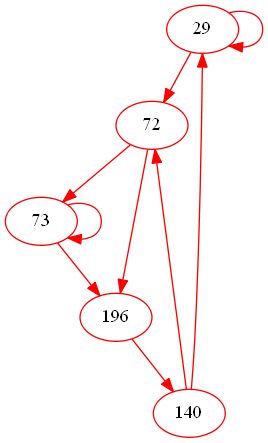
\includegraphics[width=0.7\textwidth]{fig/graph_knot256_ddt.PNG}
	\caption{the differential iterative structure $G^{IS}_{F,2}$ for KNOT-permutation-256} \label{fig:graph_knot256_ddt}
\end{figure}

\begin{figure}
	\centering
	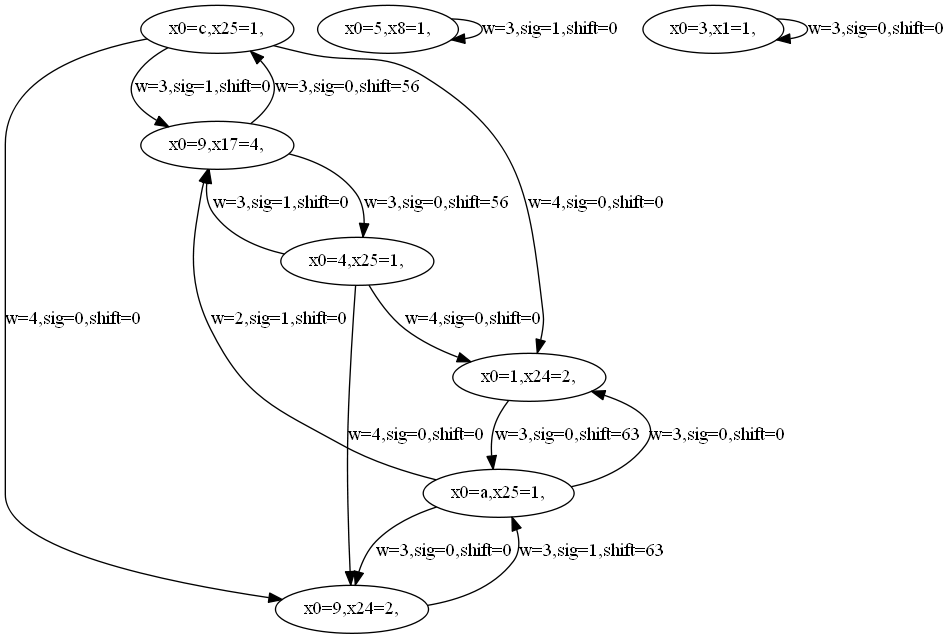
\includegraphics[width=0.7\textwidth]{fig/graph_knot256_lat.PNG}
	\caption{the linear iterative structure $G^{IS}_{F,2}$ of KNOT-permutation-256} \label{fig:graph_knot256_lat}
\end{figure}
\begin{figure}
	\centering
	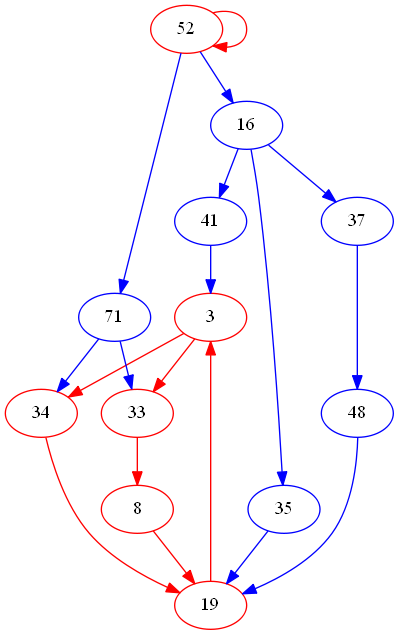
\includegraphics[width=0.7\textwidth]{fig/graph_rect_ddt.PNG}
	\caption{the differential iterative structure $G^{IS}_{F,2}$ of RECTANGLE} \label{fig:graph_rect_ddt}
\end{figure}

\begin{figure}
	\centering
	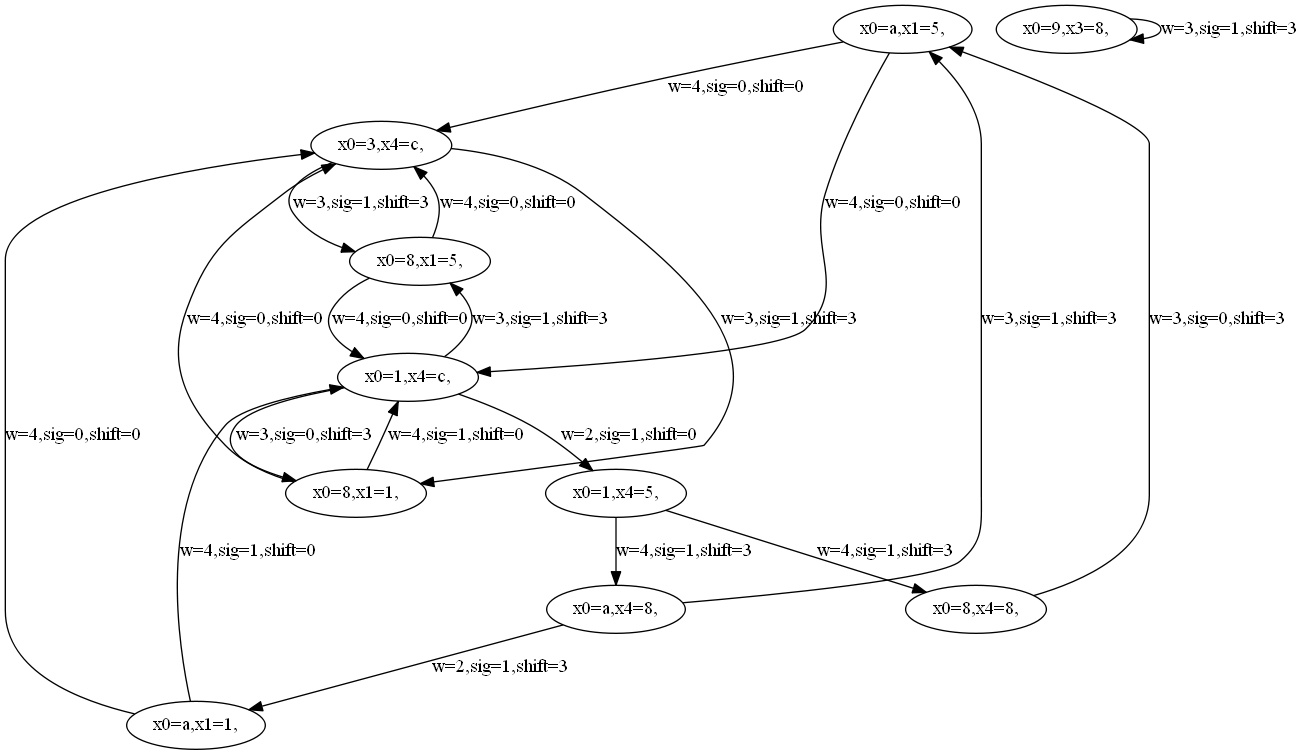
\includegraphics[width=0.7\textwidth]{fig/graph_rect_lat.PNG}
	\caption{the linear iterative structure $G^{IS}_{F,2}$ of RECTANGLE} \label{fig:graph_rect_lat}
\end{figure}

\begin{figure}
	\centering
	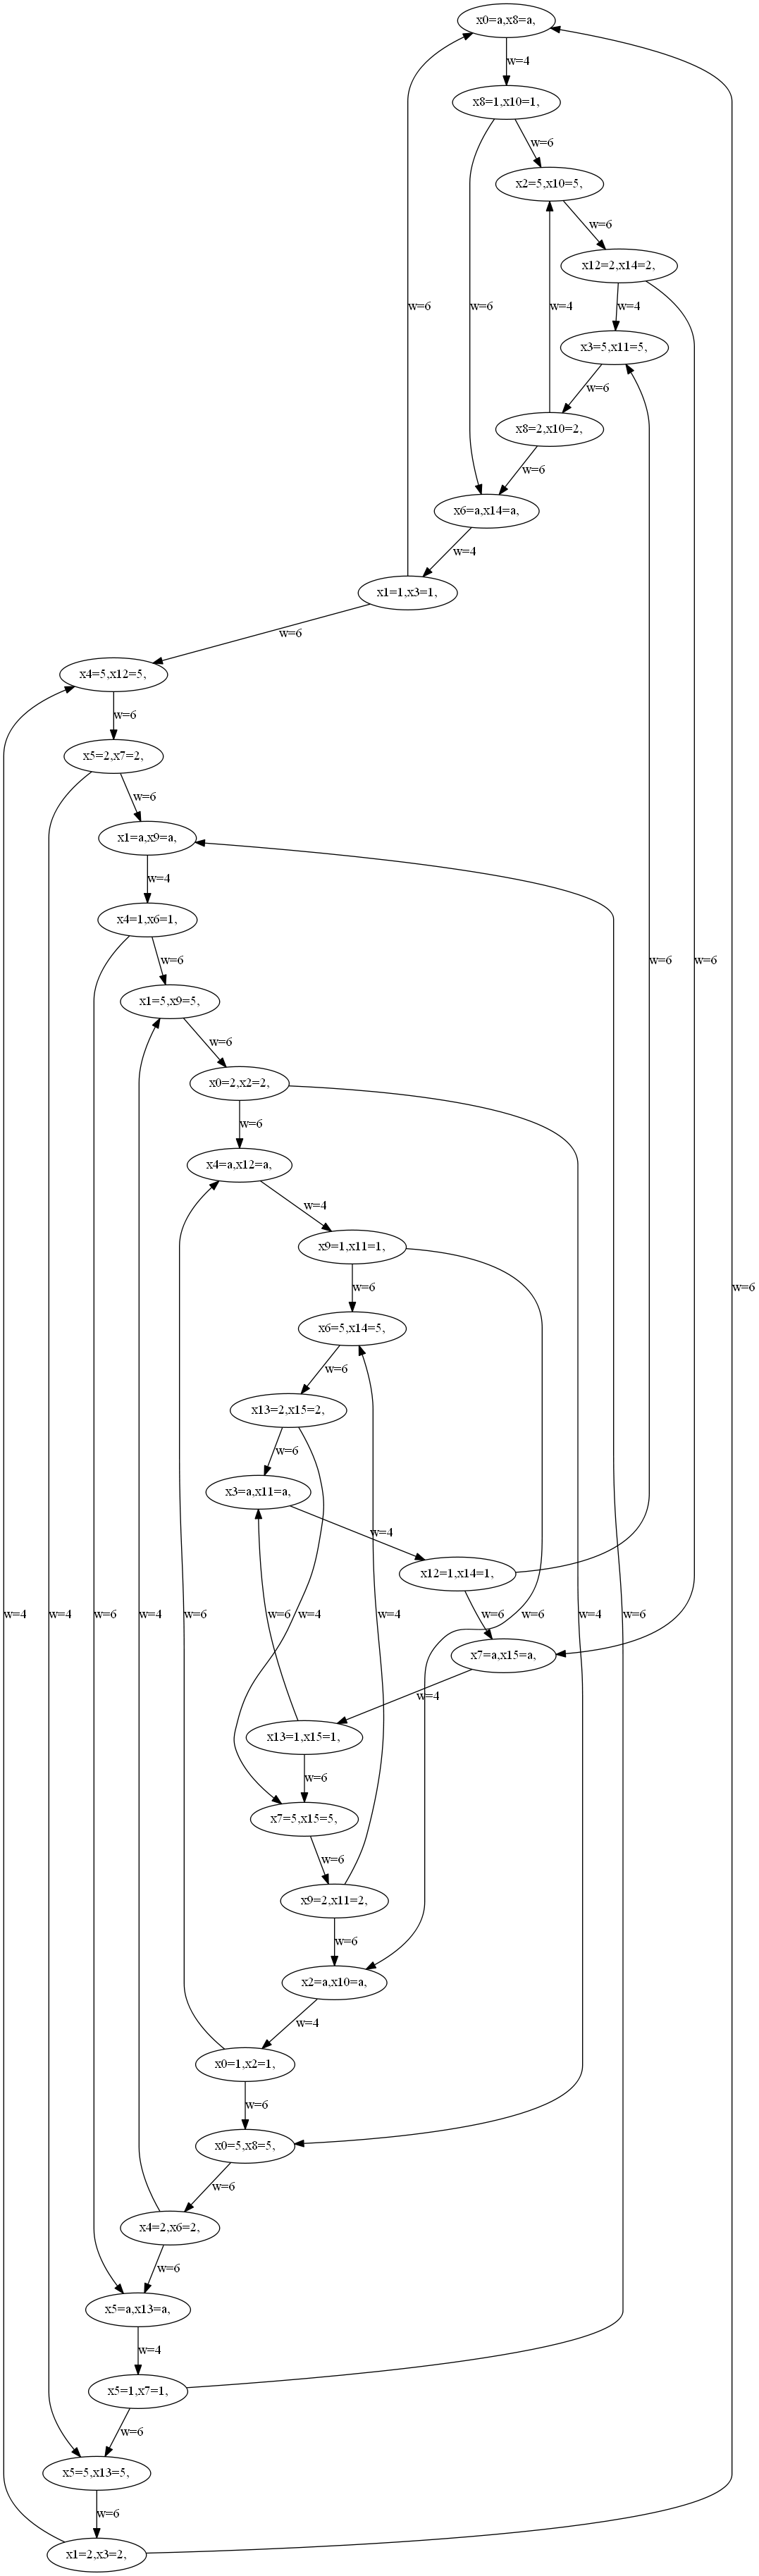
\includegraphics[width=0.4\textwidth]{fig/graph_gift_ddt.PNG}
	\caption{the differential iterative structure $G^{IS}_{F,2}$ of GIFT} \label{fig:graph_gift_ddt}
\end{figure}

\begin{figure}
	\centering
	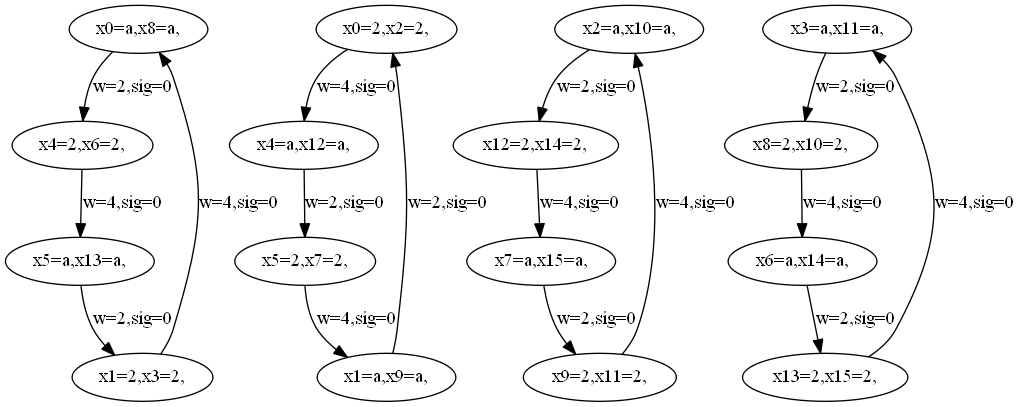
\includegraphics[width=0.7\textwidth]{fig/graph_gift_lat.PNG}
	\caption{the linear iterative structure $G^{IS}_{F,2}$ of GIFT} \label{fig:graph_gift_lat}
\end{figure}



\end{document}
